\documentclass[12pt]{article}
\usepackage[dvipsnames,table]{xcolor}
\usepackage{amsmath}
\usepackage{bbding}
\usepackage{amssymb}
\usepackage{makecell}
\usepackage[a4paper, margin=0.7in, bottom=25mm, top=16mm, headsep=0mm]{geometry}
\usepackage{import}
\usepackage{pdfpages}
\usepackage{transparent}
\usepackage{xcolor}
\usepackage{minted}
\usepackage{hyperref}
\usepackage{longtable}
\usepackage{fontspec}

\newfontfamily{\meme}{Comic Papyrus}[Extension = .ttf] 

\newcommand{\incfig}[2][1]{%
    \def\svgwidth{#1\columnwidth}
    \import{./figures/}{#2.pdf_tex}
}

\newcommand{\icol}[1]{% inline column vector
  \begin{bmatrix}#1\end{bmatrix}%
}

\newenvironment{amatrix}[1]{%
	\left\[\begin{array}{@{}*{#1}{c}|c@{}}
}{%
  \end{array}\right\]
}

\usepackage{xcolor}
\hypersetup{
    colorlinks,
    linkcolor={red!50!black},
    citecolor={blue!50!black},
    urlcolor={blue!80!black}
}

\def\arraystretch{1.3}
%\pdfsuppresswarningpagegroup=1

\title{Formula Sheet EE2E11}
\author{MaybE\_Tree}
\date{2022-09-07}

\begin{document}
\maketitle
%\tableofcontents
%\vfill
%\begin{center}
%	\textit{
%	}
%\end{center}
%\pagebreak


\section{Power}
\begin{center}
		\fbox{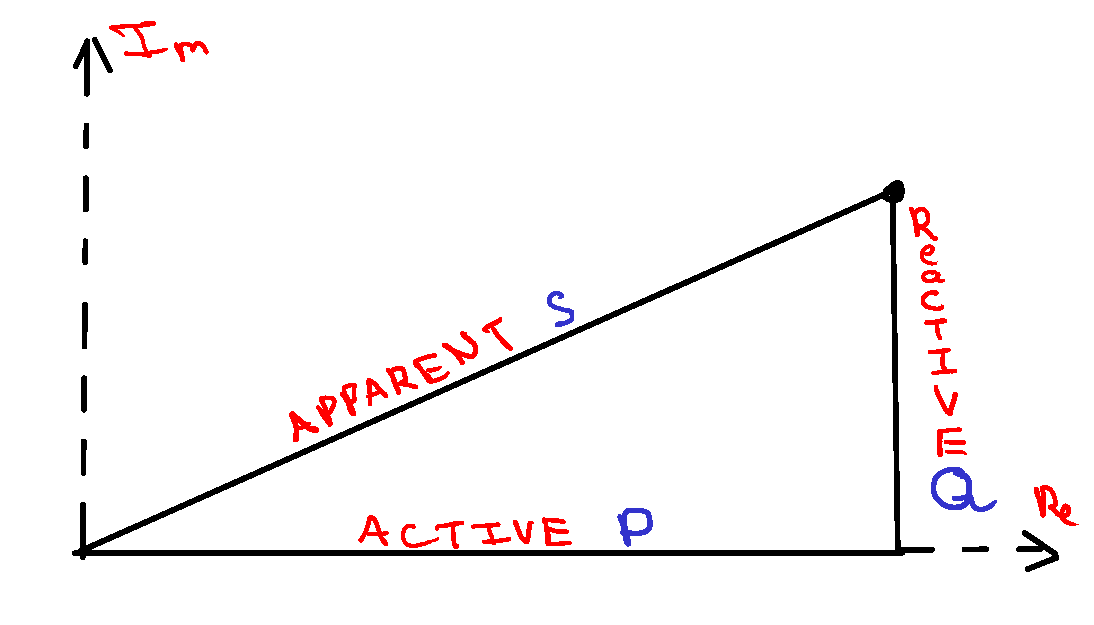
\includegraphics[width=0.6\textwidth]{xfigs/beer/beer.pdf}}
		\begin{tabular}{|cccc|}
			\hline
			\bf Name & \bf Type & \bf Symbol & \bf Unit \\\hline
			Complex Power & Complex Value & $S$ & VA \\
			Active Power & $ \text{Re}(S) $  & $P$ & W \\
			Reactive Power & $ \text{Im}(S) $  & $Q$ & VAr \\
			Apparent Power & $ |S| $  & $ |S| $  & VA \\
			\hline
		\end{tabular}
\end{center}

\subsection{Factors}
\begin{center}
	\begin{tabular}{rl}
		Power Factor &
		$ \cfrac{\text{Active Power}}{\text{Apparent Power}} = \text{Distortion Factor} * \text{Displacement Factor}$ \\
		Distortion Factor &
		$ \cfrac{\text{RMS of fundamental}}{\text{RMS of total}} = 1 \quad \text{(when no harmonics)} $ \\
		Displacement Factor &
		$ \cos \phi $, where $\phi$ is phase difference between voltage and current \\
	\end{tabular}
\end{center}
		
\section{Three-phase}
\begin{center}
		\begin{tabular}{|lcc|}
			\hline
			\bf Property & \bf Y & $ \pmb \Delta $ \\\hline
			Voltage&
			$ V_{LL} = \sqrt{3}V_\phi $ & 
			$ V_{LL} = V_\phi $ \\
			Current&
			$ I_L = I_\phi $ &
			$ I_L = \sqrt{3} I_\phi $ \\
			Phase&
			$ V_{ab} $ leads $ V_a $ by $30 ^\circ $ &
			$ I_{a} $ lags $ I_{ab} $ by $30 ^\circ $ \\
			Active Power &
			\multicolumn{2}{c|}{
				$ P = \sqrt{3}V_{LL}I_L \cos \phi $
			} \\
			Reactive Power &
			\multicolumn{2}{c|}{
				$ Q = \sqrt{3}V_{LL}I_L \sin \phi $
			} \\
			Apparent Power &
			\multicolumn{2}{c|}{
				$ |S| = \sqrt{3}V_\phi I_\phi $
			} \\
			\hline
		\end{tabular}
		\begin{itemize}
			\item All powers are given as total power
				( $ 3 * \text{Power of single load/coil}  $ )
			\item
				$ V_\phi $ is voltage across one coil.
			\item
				$ I_\phi $ is current through one coil.
			\item 
				$ \phi $  is phase difference between voltage and current
			(conventionally, voltage has 0 phase offset).
		\end{itemize}
\end{center}

\begin{longtable}{lll}
	\makecell[l]
	{
		\meme Parama's equation
	} &
	\makecell[l]
	{
		$ P = \cfrac{V}{I}  $ 
	} &
	\textit{\makecell[l]
		{
			$V$ is voltage,
			$I$ is current,
			$P$ is power.
	}} \\
\end{longtable}

\end{document}

